\chapter{Heap}

A estrutura de dados \textbf{heap} pode ser entendida como uma vetor de chaves que podem ser visto como uma árvore binária completa com uma propriedade adicional. Cada nó dessa árvore corresponde a um elemento do vetor $keys$ que armazena o valor.  Dado um vetor, podemos construir uma árvore binária completa da seguinte maneira:

\begin{minted}
[
frame=lines,
bgcolor=LightGray,
fontsize=\footnotesize,
linenos
]
{C++}
#define left(i) 2*i + 1 
#define right(i) 2*i + 2
#define parent(i) ((i-1)/2)

template <typename T> 
NodeTree<T> * createCompleteTree(vector<T> keys, int index = 0){
    if( index > keys.size()-1 )
        return nullptr;
    else{
        auto left  = createCompleteTree(keys, left(index)); 
        auto right = createCompleteTree(keys, right(index));
        return new NodeTree(keys[index], left, right);
    }
} 
\end{minted}

Utilizando o algoritmo acima, o conjunto de chaves $keys = \{30,10,45,78,12,63,36\}$

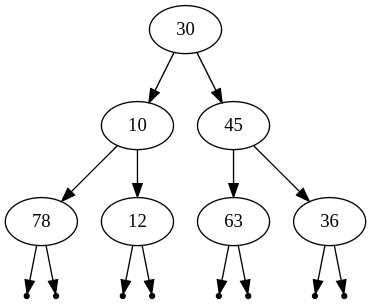
\includegraphics[width=.6\textwidth]{images/heap.png}

Queremos que o valor associado a cada nó da árvore binária seja menor que o valor do associado ao seu nó pai.

Essa propriedade pode ser verificada checando:

$$
keys[ parent(i) ] \geq keys[i] \quad \forall i \in [1,\ldots, keys.size()-1]
$$

\section{Função heapify}

A função heapify é uma subrotina responsável para construção de um heap máximo. Ela recebe como entrada um vetor arr, o tamanho atual do heap (heapsize) e um inteiro $i$. Assumimos que as árvores binárias com raiz left(i) e right(i) são heap máximos, mas que $arr[i]$ pode estar violando a propriedade de heap máximo. Se a propriedade de heap máximo for violada, colocamos o maior valor para a raiz da árvore com raiz no índice $i$ e descemos o valor $arr[i]$ para um dos seus filhos. Com a descida do valor $arr[i]$ para um dos filhos, a subárvore com a raiz nesse filho pode ter a sua propriedade violada. Como a árvore binária induzida pelo vetor de valores possui uma altura $O(log n)$. A função heapify executa no tempo $O(log~ n)$


\begin{minted}
[
frame=lines,
bgcolor=LightGray,
fontsize=\footnotesize,
linenos
]
{C++}
void heapify(vector<int> & arr, int heapsize, int i){
    int l = left(i);
    int r = right(i);
    int maior;
    cout << "heapify" << i << endl;
    if( l < heapsize && arr[l] > arr[i]){
        maior = l;
    }else{
        maior = i;
    }
    
    if(r < heapsize && arr[r] > arr[maior]){
        maior = r;
    }
    if(maior != i ){
        swap(arr[maior], arr[i]);
        heapify(arr, heapsize, maior);
    }
}
\end{minted}

\section{build heap}

A função build heap é uma função responsável por converter um vector arr de tamanho arr.size() em um heap máximo. Como a função heapify assume que as subárvores binárias construídas pelos índices left(i) e right(i) precisam ser heap máximos. O processo de construção será realizado de baixo para cima. Na árvore binária completa inicial, temos que $\lceil n/2 \rceil$ são folhas, ou seja, são subárvores que representam heap máximos. A quantidade de nós internos em uma árvore binária completa é $\lfloor n/2 \rfloor$.

\begin{minted}
[
frame=lines,
bgcolor=LightGray,
fontsize=\footnotesize,
linenos
]
{C++}
void build_heap(vector <int> & arr, int heapsize)
{
    for(int i = floor(heapsize/2); i >= 0; i--){
        heapify(arr, heapsize, i);
    }
}

\end{minted}

\fcolorbox{black}{lightblue}{
\begin{minipage}{\textwidth}
Prove que em uma árvore binária completa com $n$ nós possui $\lceil n/2 \rceil$ folhas.
\begin{proof}
Vamos provar por indução no número de nós da nossa árvore completa. Uma árvore binária completa com 1 nó possui $\lceil n/2 \rceil$ folhas. Por hipótese, assumimos que uma árvore de k nós possui $\lceil k/2 \rceil$.Seja $T$ uma árvore binária completa de k+1 nós. Seja $T_1$ e $T_2$ as subárvores binárias de T. Seja r o número de nós de $T_1$ e s o número de nós de $T_2$. Como T é uma árvore binária completa então $T_1$ ou $T_2$ são árvore binárias completas perfeitas, ou seja, todos os níveis estão completos. O número de nós de uma árvore binária completa perfeita é sempre ímpar (Cheque isso!!). Precisamos considerar 3 casos:
\begin{enumerate}
    \item r é ímpar ou s é impar.
    \item r á par e s ímpar
    \item r é impar e s á par.
\end{enumerate}

O número de folhas de uma árvore T é igual ao número de folhas da árvore $T_1$ somado ao número de folhas de $T_2$. Logo, 

$$n(T) = n(T_1) + n(T_2) = \lceil r/2 \rceil + \lceil s/2 \rceil$$

Considerando r e s ímpares, temos: 

\begin{tabular}{lll}

$\lceil r/2 \rceil$ + $\lceil s/2 \rceil$     &  = & $\lceil (r+1)/2 \rceil$ + $\lceil (s+1)/2 \rceil$\\
                                              &  = & (r+1)/2  +  (s+1)/2 \\
                                              &  = & (r+s+2)/2 \\
                                              &  = & $\lceil (r+s+1)/2 \rceil$\\
                                              &  = & $\lceil (k+1)/2 \rceil$\\
                                              &  = & $\lceil n(T)/2 \rceil$\\
                                              
                                              
\end{tabular}

Considerando r par e s ímpar, temos:

\begin{tabular}{lll}

$\lceil r/2 \rceil$ + $\lceil s/2 \rceil$     &  = & r/2  + $\lceil (s+1)/2 \rceil$\\
                                              &  = & r/2  +  (s+1)/2 \\
                                              &  = & (r+s+1)/2\\
                                              &  = & $\lceil (r+s+1)/2 \rceil$\\
                                              &  = & $\lceil (k+1)/2 \rceil$\\
                                              &  = & $\lceil n(T)/2 \rceil$\\
                                              
                                              
\end{tabular}

\end{proof}/

\end{minipage}
}
\section{heapsort}


A função heapsort recebe como entrada um vetor a ser ordenado. Inicialmente, a função build\_heap modifica o vetor para que a propriedade de heap máximo seja satisfeita. Quando a propriedade do heap é satisfeita, o elemento no índice 0 possui o maior valor. Em cada iteração, colocamos o elemento da posição zero na posição final do heap atual e decrementamos o tamanho do heap. Em seguida, utilizamos a função heapify para restaurar a propriedade de heap máximo.


\begin{minted}
[
frame=lines,
bgcolor=LightGray,
fontsize=\footnotesize,
linenos
]
{C++}
void heapsort(vector <int> & arr){
    int heapsize = arr.size();
    build_heap(arr, heapsize);
    for(int i = heapsize-1; i >= 1; i--){
        swap(arr[0], arr[i]);
        heapsize--;
        heapify(arr, heapsize, 0);
    }

}

\end{minted}

\section{Fila de prioridade}

O heap pode ser utilizado para a implementação da estrutura de dados fila de prioridade. A fila de prioridade é uma estrutura de dados que mantém um conjunto S de elementos em que cada elemento possui uma chave associada. Uma fila de prioridade $q$ máxima admite as seguintes operações:

\begin{itemize}
    \item push(x) insere um elemento x no conjunto S.
    \item top() devolve o elemento de S com a maior chave
    \item pop() remove o elemento com a maior chave
\end{itemize}

A classe priority\_queue pode ser definida da seguinte maneira:

\begin{minted}
[
frame=lines,
bgcolor=LightGray,
fontsize=\footnotesize,
linenos
]
{C++}
template <typename T>
class priority_queue{
    private:
        vector <T> arr;
        int heapsize;
        void build_heap();
        void heapify(int i);
    public:
        priority_queue() : heapsize(0){};
        priority_queue(vector <T> & v);
        void push(T value);
        void pop();
        T top();
        int size();
        bool empty();
};
\end{minted}


A função push() pode ser implementada da seguinte maneira:

\begin{minted}
[
frame=lines,
bgcolor=LightGray,
fontsize=\footnotesize,
linenos
]
{C++}
template <typename T>
void  priority_queue<T>::push(T value)
{
    if( heapsize < arr.size() ){
        arr[heapsize++] = value;
    }
    else{
        arr.push_back(value);
        heapsize++;
    }

    int i = heapsize-1;
    while( i > 0 && arr[parent(i)] < arr[i]){
        swap(arr[parent(i)], arr[i]);
        i = parent(i);
    }

}

\end{minted}

A função pop() pode ser implementada da seguinte maneira:

\begin{minted}
[
frame=lines,
bgcolor=LightGray,
fontsize=\footnotesize,
linenos
]
{C++}
template <typename T>
void priority_queue<T>::pop()
{
    if( heapsize > 0 )
    {
        arr[0] = arr[ heapsize - 1];
        heapsize--;
        heapify(0);
    }
}
\end{minted}

